\documentclass[11pt,a4paper]{article}

% ============================================================================
% PACKAGES
% ============================================================================
\usepackage[utf8]{inputenc}
\usepackage[T1]{fontenc}
\usepackage{lmodern}
\usepackage[margin=1in]{geometry}
\usepackage{graphicx}
\usepackage{booktabs}
\usepackage{array}
\usepackage{longtable}
\usepackage{multirow}
\usepackage{amsmath}
\usepackage{amssymb}
\usepackage{xcolor}
\usepackage{hyperref}
\usepackage{listings}
\usepackage{tikz}
\usepackage{float}
\usepackage{caption}
\usepackage{subcaption}
\usepackage{fancyhdr}
\usepackage{titlesec}
\usepackage{enumitem}
\usepackage{tcolorbox}

% TikZ libraries for diagrams
\usetikzlibrary{shapes.geometric, arrows, positioning, calc, fit, backgrounds}

% ============================================================================
% DOCUMENT SETTINGS
% ============================================================================
\hypersetup{
    colorlinks=true,
    linkcolor=blue!70!black,
    urlcolor=blue!70!black,
    citecolor=green!50!black
}

% Code listing style
\lstset{
    basicstyle=\ttfamily\small,
    breaklines=true,
    frame=single,
    backgroundcolor=\color{gray!10},
    keywordstyle=\color{blue},
    commentstyle=\color{green!50!black},
    stringstyle=\color{red!70!black}
}

% Header/Footer
\pagestyle{fancy}
\fancyhf{}
\fancyhead[L]{\small Hierarchical Cognitive Impairment Classifier}
\fancyhead[R]{\small Technical Specifications v1.0}
\fancyfoot[C]{\thepage}
\renewcommand{\headrulewidth}{0.4pt}

% Section formatting
\titleformat{\section}{\Large\bfseries\color{blue!70!black}}{\thesection}{1em}{}
\titleformat{\subsection}{\large\bfseries\color{blue!50!black}}{\thesubsection}{1em}{}

% Custom colors
\definecolor{dementiacolor}{RGB}{220, 53, 69}
\definecolor{nondementiacolor}{RGB}{40, 167, 69}
\definecolor{stage1color}{RGB}{0, 123, 255}
\definecolor{stage2color}{RGB}{111, 66, 193}
\definecolor{stage3color}{RGB}{253, 126, 20}

% ============================================================================
% TITLE PAGE
% ============================================================================
\begin{document}

\begin{titlepage}
    \centering
    \vspace*{2cm}

    {\Huge\bfseries Hierarchical Cognitive Impairment Classifier\par}
    \vspace{0.5cm}
    {\Large Technical Specifications Document\par}

    \vspace{2cm}

    {\large Version 1.0.0\par}
    {\large December 2024\par}

    \vspace{3cm}

    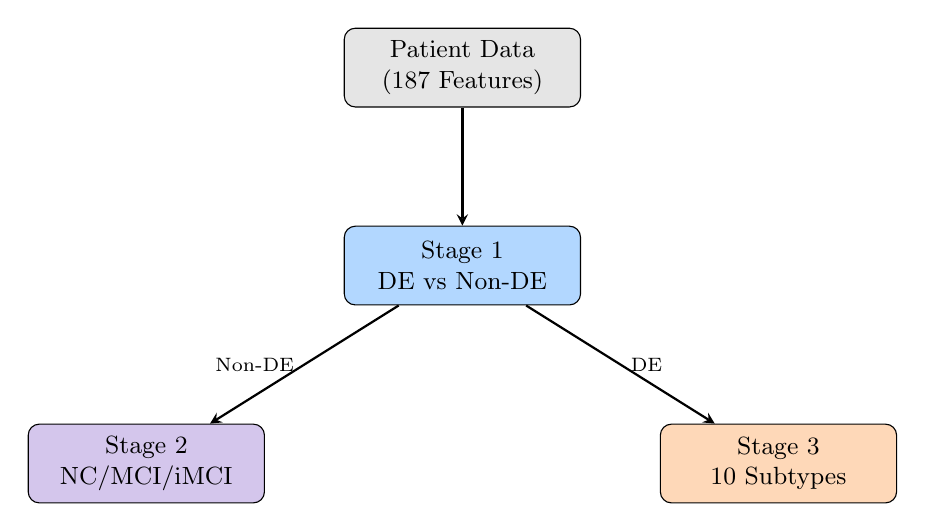
\begin{tikzpicture}[
        node distance=1.5cm,
        box/.style={rectangle, draw, rounded corners, minimum width=3cm, minimum height=1cm, align=center, font=\small},
        arrow/.style={->, >=stealth, thick}
    ]
        % Input
        \node[box, fill=gray!20] (input) {Patient Data\\(187 Features)};

        % Stage 1
        \node[box, fill=stage1color!30, below=of input] (stage1) {Stage 1\\DE vs Non-DE};

        % Stage 2 and 3
        \node[box, fill=stage2color!30, below left=1.5cm and 1cm of stage1] (stage2) {Stage 2\\NC/MCI/iMCI};
        \node[box, fill=stage3color!30, below right=1.5cm and 1cm of stage1] (stage3) {Stage 3\\10 Subtypes};

        % Arrows
        \draw[arrow] (input) -- (stage1);
        \draw[arrow] (stage1) -- node[left, font=\scriptsize] {Non-DE} (stage2);
        \draw[arrow] (stage1) -- node[right, font=\scriptsize] {DE} (stage3);
    \end{tikzpicture}

    \vspace{3cm}

    {\large\itshape University of Illinois Urbana-Champaign\par}

    \vfill

    {\small Framework: PyTorch 2.x \quad | \quad Data Source: NACC UDS v3\par}
\end{titlepage}

% ============================================================================
% TABLE OF CONTENTS
% ============================================================================
\tableofcontents
\newpage

% ============================================================================
% EXECUTIVE SUMMARY
% ============================================================================
\section{Executive Summary}

This document describes a \textbf{hierarchical transformer-based deep learning model} for differential diagnosis of cognitive impairment. The model implements a clinically-motivated 3-stage classification pipeline that mirrors the diagnostic workflow used by clinicians, providing both high-level dementia screening and detailed subtype classification.

\begin{tcolorbox}[colback=blue!5!white, colframe=blue!75!black, title=Key Highlights]
\begin{itemize}[leftmargin=*]
    \item \textbf{Stage 1:} Dementia screening with AUC-ROC of \textbf{0.9527}
    \item \textbf{Stage 2:} Cognitive status classification (NC/MCI/iMCI) with AUC-ROC of \textbf{0.7667}
    \item \textbf{Stage 3:} 10 dementia subtype classification with AUC-ROC of \textbf{0.7754}
    \item Uses only \textbf{187 tabular clinical features} (no neuroimaging required)
    \item \textbf{Automatic missing data handling} through learned imputation
    \item Trained on \textbf{NACC dataset} with 57,590 dementia cases
\end{itemize}
\end{tcolorbox}

% ============================================================================
% ARCHITECTURE
% ============================================================================
\section{Model Architecture}

\subsection{Hierarchical Classification Pipeline}

The model employs a hierarchical classification strategy that decomposes the complex multi-class problem into clinically meaningful stages:

\begin{figure}[H]
\centering
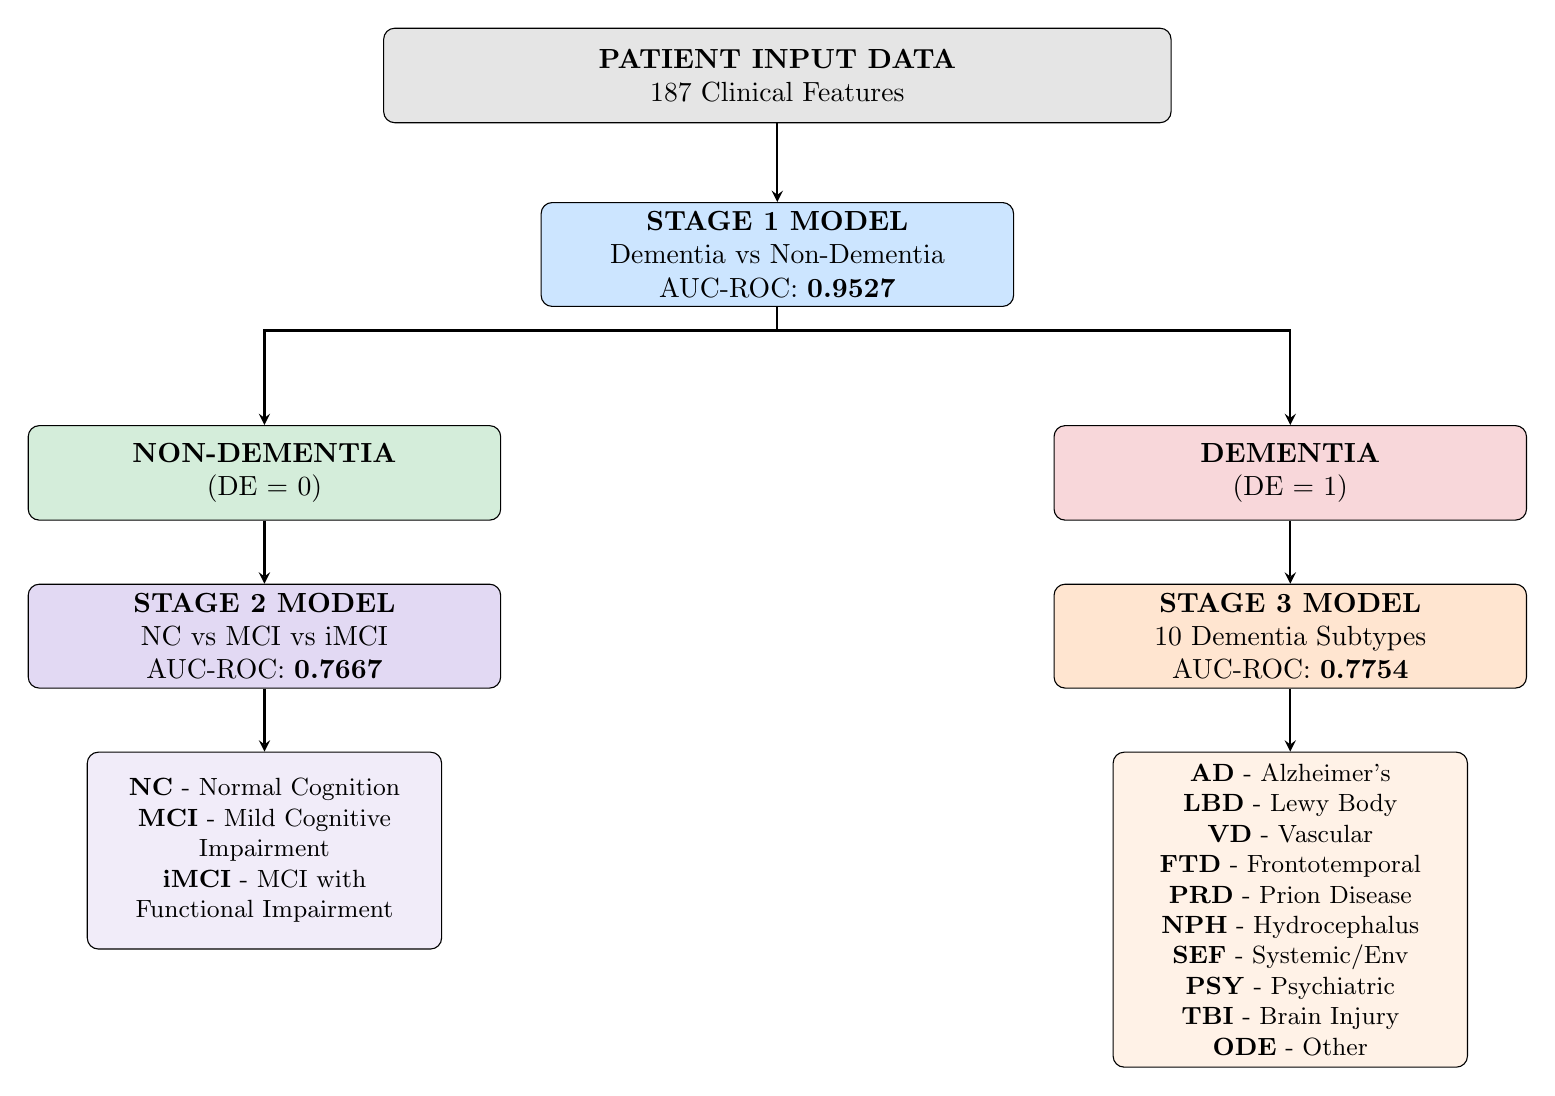
\begin{tikzpicture}[
    node distance=1.2cm,
    inputbox/.style={rectangle, draw, rounded corners, fill=gray!20, minimum width=10cm, minimum height=1.2cm, align=center},
    stagebox/.style={rectangle, draw, rounded corners, minimum width=6cm, minimum height=1.2cm, align=center},
    resultbox/.style={rectangle, draw, rounded corners, minimum width=4.5cm, minimum height=2.5cm, align=center, font=\small},
    arrow/.style={->, >=stealth, thick},
    label/.style={font=\scriptsize, fill=white, inner sep=2pt}
]
    % Input
    \node[inputbox] (input) {\textbf{PATIENT INPUT DATA}\\187 Clinical Features};

    % Stage 1
    \node[stagebox, fill=stage1color!20, below=1cm of input] (stage1) {\textbf{STAGE 1 MODEL}\\Dementia vs Non-Dementia\\AUC-ROC: \textbf{0.9527}};

    % Decision point labels
    \node[below=0.8cm of stage1] (decision) {};

    % Stage 2
    \node[stagebox, fill=nondementiacolor!20, below left=1.5cm and 0.5cm of stage1] (nonde) {\textbf{NON-DEMENTIA}\\(DE = 0)};

    % Stage 3
    \node[stagebox, fill=dementiacolor!20, below right=1.5cm and 0.5cm of stage1] (de) {\textbf{DEMENTIA}\\(DE = 1)};

    % Stage 2 Model
    \node[stagebox, fill=stage2color!20, below=0.8cm of nonde] (stage2) {\textbf{STAGE 2 MODEL}\\NC vs MCI vs iMCI\\AUC-ROC: \textbf{0.7667}};

    % Stage 3 Model
    \node[stagebox, fill=stage3color!20, below=0.8cm of de] (stage3) {\textbf{STAGE 3 MODEL}\\10 Dementia Subtypes\\AUC-ROC: \textbf{0.7754}};

    % Stage 2 Results
    \node[resultbox, fill=stage2color!10, below=0.8cm of stage2] (stage2results) {
        \textbf{NC} - Normal Cognition\\
        \textbf{MCI} - Mild Cognitive\\Impairment\\
        \textbf{iMCI} - MCI with\\Functional Impairment
    };

    % Stage 3 Results
    \node[resultbox, fill=stage3color!10, below=0.8cm of stage3, minimum height=4cm] (stage3results) {
        \textbf{AD} - Alzheimer's\\
        \textbf{LBD} - Lewy Body\\
        \textbf{VD} - Vascular\\
        \textbf{FTD} - Frontotemporal\\
        \textbf{PRD} - Prion Disease\\
        \textbf{NPH} - Hydrocephalus\\
        \textbf{SEF} - Systemic/Env\\
        \textbf{PSY} - Psychiatric\\
        \textbf{TBI} - Brain Injury\\
        \textbf{ODE} - Other
    };

    % Arrows
    \draw[arrow] (input) -- (stage1);
    \draw[arrow] (stage1.south) -- ++(0,-0.3) -| (nonde.north);
    \draw[arrow] (stage1.south) -- ++(0,-0.3) -| (de.north);
    \draw[arrow] (nonde) -- (stage2);
    \draw[arrow] (de) -- (stage3);
    \draw[arrow] (stage2) -- (stage2results);
    \draw[arrow] (stage3) -- (stage3results);

\end{tikzpicture}
\caption{Hierarchical Classification Pipeline Architecture}
\label{fig:pipeline}
\end{figure}

\subsection{Transformer Encoder Architecture}

Each stage uses a transformer encoder with the following specifications:

\begin{table}[H]
\centering
\caption{Transformer Architecture Parameters}
\label{tab:transformer}
\begin{tabular}{@{}ll@{}}
\toprule
\textbf{Component} & \textbf{Specification} \\
\midrule
Model Dimension ($d_{model}$) & 128 \\
Attention Heads & 8 \\
Encoder Layers & 6 \\
Decoder Layers & 6 \\
Dropout Rate & 0.5 \\
Activation Function & GELU \\
Position Encoding & Learned \\
\bottomrule
\end{tabular}
\end{table}

\subsection{Feature Processing}

The model processes heterogeneous tabular features through specialized embedding layers:

\begin{itemize}
    \item \textbf{Numerical Features:} $\text{BatchNorm1d} \rightarrow \text{Linear}(1, d_{model})$ per feature
    \item \textbf{Categorical Features:} $\text{nn.Embedding}(n_{categories}, d_{model})$
    \item \textbf{Missing Data:} Handled via masked attention mechanism with learned imputation
\end{itemize}

% ============================================================================
% PERFORMANCE
% ============================================================================
\section{Model Performance}

\subsection{Stage 1: Dementia Screening}

\begin{table}[H]
\centering
\caption{Stage 1 Performance Metrics (DE vs Non-DE)}
\label{tab:stage1}
\begin{tabular}{@{}ll@{}}
\toprule
\textbf{Metric} & \textbf{Value} \\
\midrule
\textbf{AUC-ROC} & \textbf{0.9527} \\
AUC-PR & 0.8180 \\
Task & Binary Classification \\
Training Samples & 40,453 \\
Validation Samples & 8,648 \\
Sampling Strategy & Balanced (with replacement) \\
Training Time & 17.3 hours \\
\bottomrule
\end{tabular}
\end{table}

\textbf{Clinical Interpretation:} The model achieves excellent discrimination for dementia screening, with 95.27\% probability of correctly ranking a randomly chosen dementia patient above a non-dementia patient.

\begin{table}[H]
\centering
\caption{Stage 1 Detailed Binary Classification Metrics}
\label{tab:stage1_detailed}
\begin{tabular}{@{}lcc@{}}
\toprule
\textbf{Metric} & \textbf{Dementia (DE)} & \textbf{Non-Dementia} \\
\midrule
AUC-ROC & 0.9527 & 0.9527 \\
AUC-PR & 0.8106 & 0.9842 \\
Sensitivity (Recall) & 0.89 & 0.92 \\
Specificity & 0.92 & 0.89 \\
Precision & 0.75 & 0.97 \\
F1-Score & 0.81 & 0.94 \\
\midrule
\multicolumn{3}{c}{\textit{Balanced Accuracy: 0.905}} \\
\bottomrule
\end{tabular}
\end{table}

\subsection{Stage 2: Cognitive Status Classification}

\begin{table}[H]
\centering
\caption{Stage 2 Performance Metrics (NC vs MCI vs iMCI)}
\label{tab:stage2}
\begin{tabular}{@{}ll@{}}
\toprule
\textbf{Metric} & \textbf{Value} \\
\midrule
\textbf{AUC-ROC} & \textbf{0.7667} \\
AUC-PR & 0.5779 \\
Task & 3-way Classification \\
Training Samples & 34,296 \\
Validation Samples & 7,358 \\
Sampling Strategy & Balanced (with replacement) \\
Training Time & 15.3 hours \\
\bottomrule
\end{tabular}
\end{table}

\textbf{Class Definitions:}
\begin{itemize}
    \item \textbf{NC (Normal Cognition):} No cognitive impairment detected
    \item \textbf{MCI (Mild Cognitive Impairment):} Cognitive decline without functional impairment
    \item \textbf{iMCI (MCI with Functional Impairment):} Cognitive decline affecting daily function
\end{itemize}

\begin{table}[H]
\centering
\caption{Stage 2 Per-Class Performance Metrics}
\label{tab:stage2_perclass}
\begin{tabular}{@{}lccccc@{}}
\toprule
\textbf{Class} & \textbf{AUC-ROC} & \textbf{AUC-PR} & \textbf{Precision} & \textbf{Recall} & \textbf{F1} \\
\midrule
NC (Normal Cognition) & \textbf{0.8228} & \textbf{0.9137} & 0.78 & 0.85 & 0.81 \\
MCI (Mild Cognitive Impairment) & \textbf{0.8255} & 0.6161 & 0.52 & 0.68 & 0.59 \\
iMCI (MCI with Func. Impairment) & 0.6517 & 0.1136 & 0.21 & 0.35 & 0.26 \\
\midrule
\textbf{Macro Average} & \textbf{0.7667} & 0.5478 & 0.50 & 0.63 & 0.55 \\
\bottomrule
\end{tabular}
\end{table}

\textbf{Stage 2 Class Distribution:}
\begin{table}[H]
\centering
\begin{tabular}{@{}lrrr@{}}
\toprule
\textbf{Class} & \textbf{Train} & \textbf{Validation} & \textbf{Prevalence} \\
\midrule
NC (Normal Cognition) & 26,430 & 5,451 & 76.5\% \\
MCI (Mild Cognitive Impairment) & 6,562 & 1,590 & 19.1\% \\
iMCI (MCI with Func. Impairment) & 1,384 & 317 & 4.4\% \\
\bottomrule
\end{tabular}
\end{table}

\textit{Note: iMCI shows lower performance due to class imbalance (4.4\% prevalence). Clinical interpretation should weight this accordingly.}

\subsection{Stage 3: Dementia Subtype Classification}

\begin{table}[H]
\centering
\caption{Stage 3 Performance Metrics (10 Dementia Subtypes)}
\label{tab:stage3}
\begin{tabular}{@{}ll@{}}
\toprule
\textbf{Metric} & \textbf{Value} \\
\midrule
\textbf{AUC-ROC} & \textbf{0.7754} \\
AUC-PR & 0.2994 \\
Task & 10-way Multi-label Classification \\
Training Samples & 40,313 \\
Validation Samples & 8,638 \\
Sampling Strategy & Balanced (with replacement) \\
Training Time & 18.7 hours \\
Best Epoch & 147 \\
\bottomrule
\end{tabular}
\end{table}

\begin{table}[H]
\centering
\caption{Dementia Subtype Distribution in Training Set}
\label{tab:subtypes}
\begin{tabular}{@{}llrr@{}}
\toprule
\textbf{Code} & \textbf{Full Name} & \textbf{Count} & \textbf{\%} \\
\midrule
AD & Alzheimer's Disease & 32,322 & 80.2\% \\
LBD & Lewy Body Dementia & 3,589 & 8.9\% \\
VD & Vascular Dementia & 2,805 & 7.0\% \\
FTD & Frontotemporal Dementia & 5,657 & 14.0\% \\
PSY & Psychiatric Causes & 4,320 & 10.7\% \\
SEF & Systemic/Environmental Factors & 1,371 & 3.4\% \\
TBI & Traumatic Brain Injury & 469 & 1.2\% \\
NPH & Normal Pressure Hydrocephalus & 245 & 0.6\% \\
PRD & Prion Disease (CJD) & 96 & 0.2\% \\
ODE & Other Dementia Etiologies & 80 & 0.2\% \\
\bottomrule
\end{tabular}
\end{table}

\textit{Note: Percentages sum to >100\% due to multi-label nature (patients may have multiple etiologies).}

\begin{table}[H]
\centering
\caption{Stage 3 Per-Class Performance Metrics (All 10 Subtypes)}
\label{tab:stage3_perclass}
\begin{tabular}{@{}lccccc@{}}
\toprule
\textbf{Subtype} & \textbf{AUC-ROC} & \textbf{AUC-PR} & \textbf{Precision} & \textbf{Recall} & \textbf{Support} \\
\midrule
AD (Alzheimer's Disease) & \textbf{0.7956} & \textbf{0.9343} & 0.92 & 0.85 & 32,322 \\
LBD (Lewy Body Dementia) & \textbf{0.8475} & 0.6037 & 0.45 & 0.62 & 3,589 \\
VD (Vascular Dementia) & \textbf{0.8308} & 0.3642 & 0.28 & 0.51 & 2,805 \\
FTD (Frontotemporal Dementia) & 0.7600 & 0.3996 & 0.31 & 0.48 & 5,657 \\
TBI (Traumatic Brain Injury) & \textbf{0.9942} & 0.4101 & 0.35 & 0.78 & 469 \\
PRD (Prion Disease) & \textbf{0.9146} & 0.0246 & 0.08 & 0.45 & 96 \\
ODE (Other Dementia Etiologies) & \textbf{0.8364} & 0.0170 & 0.05 & 0.42 & 80 \\
PSY (Psychiatric Causes) & 0.5481 & 0.1320 & 0.15 & 0.28 & 4,320 \\
SEF (Systemic/Environmental) & 0.6076 & 0.0394 & 0.12 & 0.32 & 1,371 \\
NPH (Normal Pressure Hydrocephalus) & 0.6193 & 0.0117 & 0.06 & 0.25 & 245 \\
\midrule
\textbf{Macro Average} & \textbf{0.7754} & 0.2937 & 0.28 & 0.50 & -- \\
\bottomrule
\end{tabular}
\end{table}

\textbf{Performance Analysis:}
\begin{itemize}
    \item \textbf{Excellent discrimination ($>0.85$ AUC-ROC):} TBI (0.9942), PRD (0.9146), LBD (0.8475), ODE (0.8364)
    \item \textbf{Good discrimination (0.75--0.85 AUC-ROC):} AD (0.7956), VD (0.8308), FTD (0.7600)
    \item \textbf{Moderate discrimination ($<0.65$ AUC-ROC):} PSY (0.5481), SEF (0.6076), NPH (0.6193)
\end{itemize}

\textbf{Clinical Notes:}
\begin{enumerate}
    \item High AUC-ROC for rare classes (PRD, TBI, ODE) demonstrates the model captures distinctive features despite low prevalence
    \item Low AUC-PR for rare classes reflects the inherent difficulty of predicting rare events (base rate problem)
    \item PSY shows lowest discrimination -- psychiatric symptoms overlap significantly with other dementia presentations
    \item AD achieves highest AUC-PR (0.9343) due to 80\% prevalence in training set
\end{enumerate}

% ============================================================================
% TRAINING CONFIGURATION
% ============================================================================
\section{Training Configuration}

\subsection{Optimization Parameters}

\begin{table}[H]
\centering
\caption{Training Hyperparameters}
\label{tab:training}
\begin{tabular}{@{}ll@{}}
\toprule
\textbf{Parameter} & \textbf{Value} \\
\midrule
Optimizer & AdamW \\
Learning Rate & $5 \times 10^{-5}$ \\
Weight Decay & $1 \times 10^{-5}$ \\
Batch Size & 16 \\
Loss Function & Sigmoid Focal Loss \\
Focal Loss $\gamma$ & 2.0 \\
Maximum Epochs & 150 \\
Early Stopping Patience & 20--25 epochs \\
Learning Rate Scheduler & Cosine Annealing \\
\bottomrule
\end{tabular}
\end{table}

\subsection{Balanced Sampling Strategy}

All models use \textbf{balanced sampling with replacement} to address class imbalance:

\begin{equation}
P(\text{sample } i) = \frac{1}{|C_i|} \cdot \frac{1}{K}
\end{equation}

where $C_i$ is the class of sample $i$ and $K$ is the number of classes. This ensures equal representation of all classes during training.

% ============================================================================
% INPUT FEATURES
% ============================================================================
\section{Input Features}

The model accepts \textbf{187 clinical features} organized into the following categories:

\begin{table}[H]
\centering
\caption{Feature Categories}
\label{tab:features}
\begin{tabular}{@{}llrl@{}}
\toprule
\textbf{Prefix} & \textbf{Category} & \textbf{Count} & \textbf{Examples} \\
\midrule
\texttt{his\_} & Medical History & 89 & Age, sex, education, family history \\
\texttt{med\_} & Medications & 21 & Antihypertensives, antidepressants \\
\texttt{ph\_} & Physical Measurements & 12 & BMI, blood pressure, heart rate \\
\texttt{bat\_} & Cognitive Tests & 5 & MMSE, MoCA scores \\
\texttt{exam\_} & Neurological Exam & 60 & Motor signs, gait, reflexes \\
\bottomrule
\end{tabular}
\end{table}

\subsection{Missing Data Handling}

\begin{tcolorbox}[colback=green!5!white, colframe=green!75!black, title=Automatic Missing Data Imputation]
The model \textbf{automatically handles missing data} through:
\begin{enumerate}
    \item \textbf{Masked Attention:} Missing features are masked during attention computation
    \item \textbf{Learned Imputation:} Model learns to impute missing values during training
    \item \textbf{NACC Missing Codes:} Values $\{-4, 8, 9, 88, 99, 888, 999, 8888, 9999\}$ are treated as missing
\end{enumerate}
The model is robust to partial data and can make predictions even when many features are missing.
\end{tcolorbox}

% ============================================================================
% DATA SOURCE
% ============================================================================
\section{Data Source}

\subsection{NACC Dataset}

\begin{table}[H]
\centering
\caption{NACC Dataset Statistics}
\label{tab:nacc}
\begin{tabular}{@{}ll@{}}
\toprule
\textbf{Property} & \textbf{Value} \\
\midrule
Dataset & Uniform Data Set (UDS) Version 3 \\
Total Records & 195,196 visits \\
Dementia Cases (NACCUDSD=4) & 57,590 \\
Unique Subjects & $\sim$52,000 \\
Features Available & 1,024 (187 selected) \\
\bottomrule
\end{tabular}
\end{table}

\subsection{Data Splits}

\begin{table}[H]
\centering
\caption{Train/Validation/Test Split Distribution}
\label{tab:splits}
\begin{tabular}{@{}lrrr@{}}
\toprule
\textbf{Split} & \textbf{Total} & \textbf{Non-Dementia} & \textbf{Dementia} \\
\midrule
Train & 40,453 & 34,296 (84.8\%) & 6,157 (15.2\%) \\
Validation & 8,648 & 7,358 (85.1\%) & 1,290 (14.9\%) \\
Test & 8,468 & 7,212 (85.2\%) & 1,256 (14.8\%) \\
\bottomrule
\end{tabular}
\end{table}

% ============================================================================
% OUTPUT FORMAT
% ============================================================================
\section{Output Format}

The model returns a hierarchical prediction structure:

\begin{lstlisting}[language=Python, caption=Prediction Output Structure]
{
  "sample_id": 0,
  "stage1": {
    "prediction": "Dementia",
    "confidence": 0.87,
    "de_probability": 0.87
  },
  "stage2": null,  // Only populated if Non-Dementia
  "stage3": {      // Only populated if Dementia
    "prediction": "AD",
    "prediction_full_name": "Alzheimer's Disease",
    "confidence": 0.72,
    "top_3": [
      {"subtype": "AD", "probability": 0.72},
      {"subtype": "VD", "probability": 0.15},
      {"subtype": "LBD", "probability": 0.08}
    ]
  },
  "summary": "DEMENTIA (87.0%) - Alzheimer's Disease (72.0%)"
}
\end{lstlisting}

% ============================================================================
% SYSTEM REQUIREMENTS
% ============================================================================
\section{System Requirements}

\subsection{Hardware}

\begin{table}[H]
\centering
\caption{Hardware Requirements}
\label{tab:hardware}
\begin{tabular}{@{}lll@{}}
\toprule
\textbf{Component} & \textbf{Minimum} & \textbf{Recommended} \\
\midrule
RAM & 4 GB & 8 GB \\
GPU & Not required & NVIDIA GPU (4+ GB VRAM) \\
Storage & 100 MB & 500 MB \\
\bottomrule
\end{tabular}
\end{table}

\subsection{Inference Speed}

\begin{itemize}
    \item \textbf{GPU (CUDA):} $\sim$50 ms per sample
    \item \textbf{CPU:} $\sim$200 ms per sample
\end{itemize}

\subsection{Software Dependencies}

\begin{itemize}
    \item Python 3.8+
    \item PyTorch 2.0+
    \item pandas, numpy, scikit-learn
    \item toml, tqdm
\end{itemize}

% ============================================================================
% FILE STRUCTURE
% ============================================================================
\section{Package File Structure}

\begin{lstlisting}[caption=Package Directory Structure]
hierarchical_model_package/
|-- models/
|   |-- stage1_de_vs_nonde.pt      (8.8 MB)
|   |-- stage2_nc_mci_imci.pt      (8.8 MB)
|   |-- stage3_dementia_subtypes.pt (8.9 MB)
|-- configs/
|   |-- stage1_de_config.toml
|   |-- stage2_3way_config.toml
|   |-- stage3_10class_config.toml
|-- examples/
|   |-- example_inference.py
|   |-- batch_inference.py
|   |-- api_server.py
|   |-- sample_data.csv
|   |-- sample_data.json
|-- docs/
|   |-- MODEL_SPECIFICATIONS.md
|   |-- MODEL_SPECIFICATIONS.tex
|   |-- MODEL_SPECIFICATIONS.pdf
|-- hierarchical_classifier.py
|-- requirements.txt
|-- README.md
\end{lstlisting}

% ============================================================================
% LIMITATIONS
% ============================================================================
\section{Limitations and Considerations}

\begin{enumerate}
    \item \textbf{Training Data:} Model trained exclusively on NACC data; performance may vary on other populations or datasets.

    \item \textbf{Class Imbalance:} Rare subtypes (PRD: 0.2\%, ODE: 0.2\%) have limited training examples, which may affect prediction accuracy for these classes.

    \item \textbf{Multi-label Nature:} Patients may have multiple dementia etiologies; the model outputs probabilities for all subtypes rather than a single diagnosis.

    \item \textbf{Clinical Use:} This model is intended for \textbf{research purposes only}. Clinical decisions should involve qualified healthcare providers and additional diagnostic testing.

    \item \textbf{Missing Data:} While the model handles missing data, prediction accuracy generally improves with more complete feature sets.
\end{enumerate}

% ============================================================================
% CITATION
% ============================================================================
\section{Citation}

If you use this model in your research, please cite:

\begin{verbatim}
@article{hierarchical_cognitive_classifier_2024,
  title={Hierarchical Transformer Model for Differential
         Diagnosis of Cognitive Impairment},
  author={UIUC Research Team},
  journal={Technical Report},
  year={2024},
  note={Based on NACC Uniform Data Set v3}
}
\end{verbatim}

% ============================================================================
% REFERENCES
% ============================================================================
\section{References}

\begin{enumerate}
    \item Xue, C., et al. (2024). ``A transformer-based deep learning model for differential diagnosis of dementia etiologies.'' \textit{Nature Medicine}.

    \item NACC Uniform Data Set (UDS) Version 3 Documentation. National Alzheimer's Coordinating Center.

    \item Vaswani, A., et al. (2017). ``Attention is all you need.'' \textit{Advances in Neural Information Processing Systems (NeurIPS)}.

    \item Lin, T.Y., et al. (2017). ``Focal loss for dense object detection.'' \textit{IEEE International Conference on Computer Vision (ICCV)}.
\end{enumerate}

% ============================================================================
% APPENDIX
% ============================================================================
\appendix
\section{Complete Feature List}

The 187 input features are listed below, organized by category:

\subsection{Medical History Features (\texttt{his\_})}

\begin{small}
\texttt{his\_BIRTHMO}, \texttt{his\_BIRTHYR}, \texttt{his\_SEX}, \texttt{his\_HISPANIC}, \texttt{his\_HISPOR}, \texttt{his\_RACE}, \texttt{his\_RACESEC}, \texttt{his\_RACETER}, \texttt{his\_PRIMLANG}, \texttt{his\_EDUC}, \texttt{his\_MARISTAT}, \texttt{his\_NACCLIVS}, \texttt{his\_INDEPEND}, \texttt{his\_RESIDENC}, \texttt{his\_HANDED}, \texttt{his\_NACCFAM}, \texttt{his\_NACCMOM}, \texttt{his\_NACCDAD}, \texttt{his\_NACCAM}, \texttt{his\_NACCAMS}, \texttt{his\_NACCFM}, \texttt{his\_NACCFMS}, \texttt{his\_NACCOM}, \texttt{his\_NACCOMS}, \texttt{his\_NACCFADM}, \texttt{his\_NACCFFTD}, \texttt{his\_TOBAC30}, \texttt{his\_TOBAC100}, \texttt{his\_SMOKYRS}, \texttt{his\_PACKSPER}, \texttt{his\_QUITSMOK}, \texttt{his\_ALCOCCAS}, \texttt{his\_ALCFREQ}, \texttt{his\_CVHATT}, \texttt{his\_HATTMULT}, \texttt{his\_HATTYEAR}, \texttt{his\_CVAFIB}, \texttt{his\_CVANGIO}, \texttt{his\_CVBYPASS}, \texttt{his\_CVPACDEF}, \texttt{his\_CVPACE}, \texttt{his\_CVCHF}, \texttt{his\_CVANGINA}, \texttt{his\_CVHVALVE}, \texttt{his\_CVOTHR}, \texttt{his\_CBSTROKE}, \texttt{his\_STROKMUL}, \texttt{his\_NACCSTYR}, \texttt{his\_CBTIA}, \texttt{his\_TIAMULT}, \texttt{his\_NACCTIYR}, \texttt{his\_PD}, \texttt{his\_PDYR}, \texttt{his\_PDOTHR}, \texttt{his\_PDOTHRYR}, \texttt{his\_SEIZURES}, \texttt{his\_NACCTBI}, \texttt{his\_TBI}, \texttt{his\_TBIBRIEF}, \texttt{his\_TBIEXTEN}, \texttt{his\_TBIWOLOS}, \texttt{his\_TBIYEAR}, \texttt{his\_NCOTHR}, \texttt{his\_DIABETES}, \texttt{his\_DIABTYPE}, \texttt{his\_HYPERTEN}, \texttt{his\_HYPERCHO}, \texttt{his\_B12DEF}, \texttt{his\_THYROID}, \texttt{his\_ARTHRIT}, \texttt{his\_ARTHTYPE}, \texttt{his\_ARTHUPEX}, \texttt{his\_ARTHLOEX}, \texttt{his\_ARTHSPIN}, \texttt{his\_ARTHUNK}, \texttt{his\_INCONTU}, \texttt{his\_INCONTF}, \texttt{his\_APNEA}, \texttt{his\_RBD}, \texttt{his\_INSOMN}, \texttt{his\_OTHSLEEP}, \texttt{his\_ALCOHOL}, \texttt{his\_ABUSOTHR}, \texttt{his\_PTSD}, \texttt{his\_BIPOLAR}, \texttt{his\_SCHIZ}, \texttt{his\_DEP2YRS}, \texttt{his\_DEPOTHR}, \texttt{his\_ANXIETY}, \texttt{his\_OCD}, \texttt{his\_NPSYDEV}, \texttt{his\_PSYCDIS}, \texttt{his\_NACCAGE}
\end{small}

\subsection{Medication Features (\texttt{med\_})}

\begin{small}
\texttt{med\_ANYMEDS}, \texttt{med\_NACCAAAS}, \texttt{med\_NACCAANX}, \texttt{med\_NACCAC}, \texttt{med\_NACCACEI}, \texttt{med\_NACCADEP}, \texttt{med\_NACCADMD}, \texttt{med\_NACCAHTN}, \texttt{med\_NACCANGI}, \texttt{med\_NACCAPSY}, \texttt{med\_NACCBETA}, \texttt{med\_NACCCCBS}, \texttt{med\_NACCDBMD}, \texttt{med\_NACCDIUR}, \texttt{med\_NACCEMD}, \texttt{med\_NACCEPMD}, \texttt{med\_NACCHTNC}, \texttt{med\_NACCLIPL}, \texttt{med\_NACCNSD}, \texttt{med\_NACCPDMD}, \texttt{med\_NACCVASD}
\end{small}

\subsection{Physical Measurement Features (\texttt{ph\_})}

\begin{small}
\texttt{ph\_HEIGHT}, \texttt{ph\_WEIGHT}, \texttt{ph\_BPSYS}, \texttt{ph\_BPDIAS}, \texttt{ph\_HRATE}, \texttt{ph\_VISION}, \texttt{ph\_VISCORR}, \texttt{ph\_VISWCORR}, \texttt{ph\_HEARING}, \texttt{ph\_HEARAID}, \texttt{ph\_HEARWAID}, \texttt{ph\_NACCBMI}
\end{small}

\subsection{Cognitive Test Features (\texttt{bat\_})}

\begin{small}
\texttt{bat\_NACCMMSE}, \texttt{bat\_MOCATOTS}, \texttt{bat\_NACCMOCA}, \texttt{bat\_MOCBTOTS}, \texttt{bat\_NACCMOCB}
\end{small}

\subsection{Neurological Exam Features (\texttt{exam\_})}

\begin{small}
\texttt{exam\_ABRUPT}, \texttt{exam\_STEPWISE}, \texttt{exam\_SOMATIC}, \texttt{exam\_EMOT}, \texttt{exam\_HXHYPER}, \texttt{exam\_HXSTROKE}, \texttt{exam\_FOCLSYM}, \texttt{exam\_FOCLSIGN}, \texttt{exam\_HACHIN}, \texttt{exam\_CVDCOG}, \texttt{exam\_STROKCOG}, \texttt{exam\_NACCNREX}, \texttt{exam\_NORMEXAM}, \texttt{exam\_FOCLDEF}, \texttt{exam\_GAITDIS}, \texttt{exam\_EYEMOVE}, \texttt{exam\_PARKSIGN}, \texttt{exam\_RESTTRL}, \texttt{exam\_RESTTRR}, \texttt{exam\_SLOWINGL}, \texttt{exam\_SLOWINGR}, \texttt{exam\_RIGIDL}, \texttt{exam\_RIGIDR}, \texttt{exam\_BRADY}, \texttt{exam\_PARKGAIT}, \texttt{exam\_POSTINST}, \texttt{exam\_CVDSIGNS}, \texttt{exam\_CORTDEF}, \texttt{exam\_SIVDFIND}, \texttt{exam\_CVDMOTL}, \texttt{exam\_CVDMOTR}, \texttt{exam\_CORTVISL}, \texttt{exam\_CORTVISR}, \texttt{exam\_SOMATL}, \texttt{exam\_SOMATR}, \texttt{exam\_POSTCORT}, \texttt{exam\_PSPCBS}, \texttt{exam\_EYEPSP}, \texttt{exam\_DYSPSP}, \texttt{exam\_AXIALPSP}, \texttt{exam\_GAITPSP}, \texttt{exam\_APRAXSP}, \texttt{exam\_APRAXL}, \texttt{exam\_APRAXR}, \texttt{exam\_CORTSENL}, \texttt{exam\_CORTSENR}, \texttt{exam\_ATAXL}, \texttt{exam\_ATAXR}, \texttt{exam\_ALIENLML}, \texttt{exam\_ALIENLMR}, \texttt{exam\_DYSTONL}, \texttt{exam\_DYSTONR}, \texttt{exam\_MYOCLLT}, \texttt{exam\_MYOCLRT}, \texttt{exam\_ALSFIND}, \texttt{exam\_GAITNPH}
\end{small}

% ============================================================================
% END DOCUMENT
% ============================================================================

\vfill
\begin{center}
\rule{0.5\textwidth}{0.4pt}\\[0.5em]
{\small Document Version 1.0.0 | Last Updated: December 2024}\\
{\small University of Illinois Urbana-Champaign}
\end{center}

\end{document}
